\begin{frame}{Infrastructure of Isolation: Namespace }
    \begin{itemize}
        \item A namespace wraps a global system resource.
        \pause
        \item System resource can be: cgroup,IPC,Network,Mount,PID,Time,User,TS
        \pause
        \item A process belongs to one specific namespace, and can only see resource tagged with same namespace.
    \end{itemize}
    \pause
    \begin{columns}
        \begin{column}{0.7\textwidth}
            \begin{figure}
                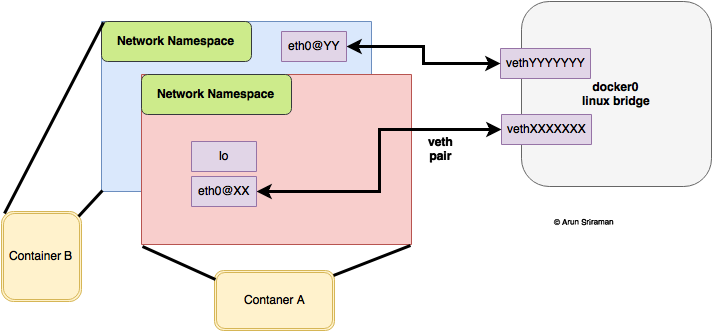
\includegraphics[width=1\textwidth]{assets/network.png}
                \caption{docker network isolation }
            \end{figure}
        \end{column}
        \begin{column}{0.3\textwidth}
            Let's take \textbf{netns} as example.
        \end{column}
    \end{columns}
\end{frame}